% Provenance (never printed): see sources/outline_sources.md (Year 2: anatexis, migmatites,
% granite types and their sources). Wet granite solidus from Stern and Wyllie (1981) and
% Boettcher and Wyllie (1968); dehydration-melting brackets from Patino Douce and Harris
% (1998), Berger and Kalt (1999), Skjerlie and Johnston (1996); water solubility from Holtz
% et al. (1995); migmatite terms from the IUGS-SCMR proposal and BGS RR 99-02; aluminosity
% after Shand (as given by Moyen et al. 2017); figure data in figdata/bachelor-2/anatexis.py
% (paths from ptpaths.py); exercise and problem values in the Book 4 scratch calculator
% calc/ch12.py.
\chapter{Pelelehan Kerak: Migmatit dan Granit}\label{ch:b2:crustal-melting}

Granitlah yang membuat benua ringan, dan mantel tidak dapat membuatnya secara langsung:
lelehan \omterm{def:b2:mantle-melting:peridotites}{peridotit} adalah basal. Sebagian besar granit adalah kerak benua yang melelehkan dirinya sendiri.
Ketika akar pegunungan yang menebal memanas, ketika basal menggenang di bawah kerak, atau ketika batuan
panas naik dan tekanannya turun, mika dan amfibol kerak dalam melepaskan
airnya, cairan granitik muncul di antara butir-butir mineral, dan batuan itu menjadi
\omterm{def:b2:crustal-melting:migmatite}{migmatit}, separuh metamorf, separuh beku. Bab ini mengikuti cairan itu dari lapisan tipis
pertamanya sampai \omterm{def:b2:magma-emplacement:bodies}{pluton} yang mungkin dibangunnya, dan membaca dalam kimia sebuah granit batuan asal
lelehannya.

\begin{recall}
\textbf{Dari volume sekolah menengah atas}: granit, granitoid, dan granodiorit; batuan felsik dan mafik;
akar sabuk pegunungan. \textbf{Dari volume Tahun 1}: produksi panas radiogenik
di kerak; hidrolisis silikat dan mineral lempung. \textbf{Dari buku-buku kimia}: solidus dan likuidus
sistem biner, massa molar dan jumlah zat. \textbf{Dari
\cref{ch:b2:magma-emplacement}}: \omterm{def:b2:magma-emplacement:bodies}{retas}, \omterm{def:b2:magma-emplacement:bodies}{pluton}, dan \omterm{def:b2:magma-emplacement:ascent}{diapir}. \textbf{Dari
\cref{ch:b2:mantle-melting}}: \omterm{def:b2:mantle-melting:melting}{pelelehan sebagian}, \omterm{def:b2:mantle-melting:peritectic}{pelelehan inkongruen}, dan \omterm{def:b2:mantle-melting:melting}{pelelehan
dekompresi}. \textbf{Dari \cref{ch:b2:metamorphic-facies}}: \omterm{def:b2:metamorphic-facies:protoliths}{metapelit}, \omterm{def:b2:metamorphic-facies:clapeyron}{kemiringan Clapeyron}
suatu reaksi, dan fasies. \textbf{Dari \cref{ch:b2:pt-paths}}: \omterm{def:b2:pt-paths:ptt}{lintasan P--T--t} dan
model penebalan kerak.
\end{recall}

\section{Mengapa kerak meleleh}\label{sec:b2:crustal-melting:why}

Istilahnya tua dan sederhana.

\begin{definition}[Anateksis]\label{def:b2:crustal-melting:anatexis}
Yang disebut \emph{anateksis}\index{anateksis} adalah pelelehan suatu batuan, berapa pun derajat pelelehannya;
dalam praktik, istilah ini dipakai untuk \omterm{def:b2:mantle-melting:melting}{pelelehan sebagian} kerak benua.
\end{definition}
% ledger: scmr:migmatite

\subsection*{Solidus basah}

Granit meleleh pada suhu rendah hanya bila basah. Stern dan Wyllie melelehkan sebuah granit
biotit dari \omterm{def:b2:magma-emplacement:bodies}{batolit} Sierra Nevada dengan air berlebih: cairan pertama muncul pada
\qty{680}{\celsius} pada \qty{2}{kbar} dan pada \qty{620}{\celsius} pada \qty{10}{kbar}, dan
seluruh batuan meleleh hanya \qty{35}{\celsius} di atas solidus pada \qty{2}{kbar}, tetapi
\qty{105}{\celsius} di atasnya pada \qty{10}{kbar}. Granit yang sama, yang diteliti lebih awal oleh
Boettcher dan Wyllie, mulai meleleh pada \qty{605}{\celsius} pada \qty{15.3}{kbar}; di dekat
\qty{17}{kbar} plagioklasnya terurai menjadi jadeit dan kuarsa, dan dari situ solidusnya
berbalik naik, mencapai \qty{670}{\celsius} pada \qty{27}{kbar}.
% ledger: sw81:wet-solidus, bw68:wet-solidus

Solidus basah turun ketika tekanan naik, kebalikan dari solidus kering. Penyebabnya adalah ke mana
air itu pergi. Air bebas adalah fluida bermassa jenis rendah; bila terlarut dalam lelehan, air hanya menempati
sedikit ruang: Holtz dan kawan-kawan mendapati volume molar parsialnya dalam lelehan granitik mendekati
\qtyrange{10}{12}{\cubic\centi\metre\per\mole}, dibandingkan dengan \qty{18}{\cubic\centi\metre\per\mole}
untuk air cair pada kondisi ruang dan lebih besar lagi untuk fluida panas. Reaksi pelelehan
\[\text{kuarsa} + \text{feldspar} + \ce{H2O}\ (\text{fluida}) \longrightarrow
\text{lelehan hidrus}\]
karena itu memiliki perubahan volume negatif, sedangkan perubahan entropinya, seperti pada setiap pelelehan,
positif: menurut relasi Clapeyron \cref{ch:b2:metamorphic-facies}, kemiringannya
$\mathrm{d}P/\mathrm{d}T = \Delta S/\Delta V$ negatif. Tekanan juga memungkinkan lebih banyak air
masuk ke dalam lelehan: untuk lelehan haplogranit pada \qty{800}{\celsius}, kadar jenuhnya naik
dari \qty{2.80}{\percent} massa pada \qty{0.5}{kbar} menjadi \qty{9.97}{\percent} pada
\qty{5}{kbar} dan \qty{13.82}{\percent} pada \qty{8}{kbar}, sekitar \qty{1.27}{\percent} lebih banyak
per kilobar antara 3 dan \qty{8}{kbar}.
% ledger: holtz95:solubility

\begin{omfigure}
\centering
\begin{tikzpicture}
\begin{axis}[omrecord, width=0.5\linewidth, height=4.8cm,
  xmin=0, xmax=9, ymin=0, ymax=15, xlabel={$P$ (\unit{kbar})},
  ylabel={\ce{H2O} dalam lelehan (\unit{\percent})},
  tick label style={font=\scriptsize}, label style={font=\small}]
\addplot[only marks, mark=*, mark size=1.6pt, blue!70!black]
  table[x=P_kbar, y=H2O_wt] {figdata/out/bachelor-2-anatexis-water.dat};
\addplot[thick, red!75!black] table[x=P_kbar, y=H2O_wt] {figdata/out/bachelor-2-anatexis-waterfit.dat};
\end{axis}
\end{tikzpicture}
\par\smallskip{\small Air yang dapat dilarutkan lelehan haplogranit pada \qty{800}{\celsius}
(titik terukur); merah: garis kuadrat terkecil melalui titik-titik dari 3 sampai
\qty{8}{kbar}, kemiringan \qty{1.26}{\percent} per kilobar.}
\end{omfigure}
% ledger: holtz95:solubility

Akan tetapi, kerak dalam hanya mengandung sedikit air bebas: batuan metamorf yang telah terpanaskan
sudah mengusir sebagian besar air porinya, melalui reaksi dehidrasi
\cref{ch:b2:metamorphic-facies}. Airnya kini terkunci dalam mika dan amfibol. Pelelehan
lalu harus menunggu mineral-mineral itu sendiri terurai.

\begin{definition}[Pelelehan dengan fluida dan pelelehan dehidrasi]\label{def:b2:crustal-melting:reactions}
Yang disebut \emph{pelelehan dengan fluida}\index{pelelehan dengan fluida} (atau pelelehan berfluks air) adalah
pelelehan dengan kehadiran fluida berair bebas, pada atau di dekat solidus basah; lelehan
yang dihasilkan dibatasi oleh pasokan fluida. Yang disebut \emph{pelelehan dehidrasi}\index{pelelehan dehidrasi} (pelelehan tanpa fluida) adalah
\omterm{def:b2:mantle-melting:peritectic}{pelelehan inkongruen} suatu mineral hidrus, mika atau
amfibol, bersama kuarsa dan feldspar, tanpa fluida bebas sama sekali: air mineral itu
masuk ke dalam lelehan, dan mineral anhidrat baru (K-feldspar peritektik, aluminosilikat,
garnet, kordierit, ortopiroksen) tumbuh di sampingnya.
\end{definition}
% ledger: pj98:productivity, koester02:melting, pdh98:himalaya

Percobaan menetapkan di mana setiap mineral hidrus menyerah. Pada sekis muskovit dari
Himalaya, Patiño Douce dan Harris mendapati \omterm{def:b2:crustal-melting:reactions}{pelelehan dehidrasi} dimulai pada 750 sampai
\qty{800}{\celsius} antara 6 dan \qty{10}{kbar}; air yang ditambahkan pada batuan yang sama menurunkan
solidusnya tetapi menghasilkan lelehan trondhjemitik yang tidak mirip \omterm{def:b2:crustal-melting:leucogranite}{leukogranit}. Sebuah gneis semipelitik
mulai meleleh di dekat \qty{700}{\celsius} melalui muskovit fengitiknya, tetapi menghasilkan kurang
dari \qty{9}{\percent} lelehan; di atas \qty{800}{\celsius}, penguraian biotit dan
kordierit menghasilkan 10 sampai \qty{63}{\percent} volume. \omterm{def:b2:crustal-melting:reactions}{Pelelehan dehidrasi} biotit terjadi
pada 800 sampai \qty{850}{\celsius} dan 0.5 sampai \qty{0.7}{GPa} di \omterm{def:b2:crustal-melting:migmatite}{migmatit}
Bayerische Wald, dan amfibol menambahkan sekitar \qty{25}{\percent} volume lelehan antara 875
dan \qty{925}{\celsius} pada 10 sampai \qty{12.5}{kbar}. Urutannya adalah urutan kuatnya ikatan air:
muskovit lebih dulu, biotit berikutnya, amfibol terakhir.
% ledger: pdh98:himalaya, koester02:melting, bk99:migmatites, sj96:amphibole, moyen17:aluminosity

\begin{proposition}[Fraksi lelehan yang dibatasi air]\label{prop:b2:crustal-melting:water}
Dalam \omterm{def:b2:crustal-melting:reactions}{pelelehan dehidrasi} tanpa fluida bebas, jika suatu batuan mengandung fraksi massa $X$ suatu
mineral hidrus yang mengandung fraksi massa $w$ air, dan jika seluruh air ini masuk ke dalam
lelehan yang mengandung fraksi massa $c$ air, maka fraksi massa lelehannya adalah
\[F = \frac{X\,w}{c}.\]
Karena $c$ tidak dapat melebihi kadar jenuh $c_{\mathrm{sat}}$ pada tekanan dan
suhu pelelehan, $F \ge X\,w/c_{\mathrm{sat}}$: makin sedikit air yang dikandung lelehan, makin
banyak lelehan yang dihasilkan oleh mika yang sama.
\end{proposition}

\begin{proof}
Setiap kilogram batuan, mineral itu melepaskan $X\,w$ kilogram air. Tanpa fase fluida
dan tanpa air yang tersisa dalam padatan, semuanya berada dalam lelehan, yang massanya $F$ mengandung $c\,F$
kilogram air: $c\,F = X\,w$. Karena $c \le c_{\mathrm{sat}}$, $F = Xw/c \ge
Xw/c_{\mathrm{sat}}$.
\end{proof}

Muskovit, \ce{KAl3Si3O10(OH)2} dengan massa molar \qty{398.3}{\gram\per\mole}, mengandung dua
gugus hidroksil, setara dengan satu molekul air, atau \qty{4.52}{\percent} massanya.
Sekis dengan \qty{20}{\percent} muskovit karena itu memiliki \qty{9.0}{\gram} air
per kilogram untuk dilepaskan; bila terlarut dengan kadar \qty{6}{\percent}, air itu menghasilkan \qty{150}{\gram}
lelehan. Mika menetapkan anggarannya, itulah sebabnya kerak subur, yaitu kerak yang mudah meleleh,
kaya akan mika: \omterm{def:b2:metamorphic-facies:protoliths}{metapelit} yang terutama.

\begin{omfigure}
\centering
\begin{tikzpicture}
\begin{axis}[omrecord, width=0.8\linewidth, height=7cm,
  xmin=500, xmax=1000, ymin=0, ymax=20, xlabel={$T$ (\unit{\celsius})}, ylabel={$P$ (\unit{kbar})},
  tick label style={font=\scriptsize}, label style={font=\small}, clip=false]
\addplot[fill=orange!35, draw=orange!70!black] coordinates {(750,6) (800,6) (800,10) (750,10) (750,6)};
\addplot[fill=red!25, draw=red!70!black] coordinates {(800,5) (850,5) (850,7) (800,7) (800,5)};
\addplot[fill=green!25, draw=green!50!black] coordinates {(875,10) (925,10) (925,12.5) (875,12.5) (875,10)};
\node[font=\scriptsize, orange!50!black, align=center] at (axis cs:775,8) {mus-\\kovit};
\node[font=\scriptsize, red!60!black] at (axis cs:825,4.4) {biotit};
\node[font=\scriptsize, green!35!black, anchor=west] at (axis cs:927,11.25) {amfibol};
\addplot[very thick, blue!70!black, mark=*, mark size=1.5pt]
  table[x=T_C, y=P_kbar] {figdata/out/bachelor-2-anatexis-solidi.dat};
\node[font=\scriptsize, blue!70!black, anchor=west] at (axis cs:612,15.6) {solidus granit basah};
\addplot[thick, black, postaction={decorate}, decoration={markings,
  mark=at position 0.3 with {\arrow{>}}, mark=at position 0.75 with {\arrow{>}}}]
  table[x=T_C, y=P_kbar, restrict x to domain=500:1000,
  restrict expr to domain={\thisrow{t_Myr}}{0:100}] {figdata/out/bachelor-2-anatexis-path35.dat};
\node[font=\scriptsize, anchor=north] at (axis cs:560,4.2) {batuan dari \qty{35}{km}};
\addplot[thick, dashed, black, postaction={decorate}, decoration={markings,
  mark=at position 0.3 with {\arrow{>}}, mark=at position 0.7 with {\arrow{>}}}]
  table[x=T_C, y=P_kbar, restrict x to domain=500:1000,
  restrict expr to domain={\thisrow{t_Myr}}{0:100}] {figdata/out/bachelor-2-anatexis-path70.dat};
\node[font=\scriptsize, anchor=south] at (axis cs:760,19.4) {dasar kerak yang menebal};
\end{axis}
\end{tikzpicture}
\par\smallskip{\small Tempat kerak meleleh. Biru: solidus granit biotit dengan
air berlebih (titik terukur, dihubungkan dengan ruas-ruas garis lurus). Kotak: kondisi tempat
\omterm{def:b2:crustal-melting:reactions}{pelelehan dehidrasi} muskovit, biotit, dan amfibol teramati dalam percobaan dan dalam
\omterm{def:b2:crustal-melting:migmatite}{migmatit}. Hitam: lintasan yang dihitung dengan model penebalan
\cref{ch:b2:pt-paths}; batuan yang berakhir pada \qty{35}{km} setelah penumpukan (garis utuh) tidak pernah
mencapai solidus basah, sedangkan dasar kerak yang menebal (garis putus-putus) melewati
\qty{900}{\celsius}. Kedua lintasan digambar untuk 100 juta tahun pertama, sampai
erosi berhenti.}
\end{omfigure}
% ledger: sw81:wet-solidus, bw68:wet-solidus, pdh98:himalaya, bk99:migmatites, sj96:amphibole, et84:ptt

\subsection*{Dari mana panasnya berasal}

Gambar di atas menetapkan masalahnya: kerak hanya meleleh di tempat suhunya lebih tinggi dari sekitar
\qty{700}{\celsius}, sedangkan geoterm tunak model dalam \cref{ch:b2:pt-paths}
hanya mencapai \qty{595}{\celsius} di dasar kerak setebal \qty{35}{km}. Ada tiga jalan
untuk melampaui reaksi \omterm{def:b2:crustal-melting:reactions}{pelelehan dehidrasi}.

\emph{Penebalan dan panas radiogenik.} Dalam model \cref{ch:b2:pt-paths}, kerak yang
digandakan oleh penumpukan memanas dari dalam; batuan yang berakhir di kedalaman kerak tengah mencapai puncak pada
\qty{593}{\celsius} dan tidak pernah meleleh, tetapi dasar kerak yang menebal melewati
\qty{800}{\celsius} setelah sekitar 31 juta tahun dan \qty{900}{\celsius} setelah sekitar 56 juta tahun, melampaui
reaksi biotit. Pelelehan kerak bawah adalah akibat lambat dari penebalan.
% ledger: et84:ptt

\emph{Dekompresi.} Batuan panas yang diangkat lebih cepat daripada mendinginnya melintasi
kurva \omterm{def:b2:crustal-melting:reactions}{pelelehan dehidrasi} dari sisi tekanan tinggi. Patiño Douce dan Harris mendapati bahwa
solidus sekis muskovit memiliki $\mathrm{d}P/\mathrm{d}T$ yang lebih kecil daripada solidus
sekis biotit, sehingga sekis muskovit lebih mudah meleleh saat dekompresi, dan
menyimpulkan bahwa \omterm{def:b2:crustal-melting:leucogranite}{leukogranit} Himalaya terbentuk melalui \omterm{def:b2:crustal-melting:reactions}{pelelehan dehidrasi} \omterm{def:b2:metamorphic-facies:protoliths}{metapelit}
selama dekompresi adiabatik pada 6 sampai \qty{8}{kbar} dan 750 sampai \qty{770}{\celsius}.
% ledger: pdh98:himalaya

\emph{Panas dari bawah.} Basal dari mantel yang berhenti di dasar kerak membawa
panasnya dan panas laten kristalisasinya.

\begin{definition}[Underplating mafik]\label{def:b2:crustal-melting:underplating}
Yang disebut \emph{underplating mafik}\index{underplating mafik} adalah penggenangan \omterm{def:b2:magma-emplacement:magma}{magma} basaltik
yang berasal dari mantel pada atau di dekat dasar kerak benua, tempat \omterm{def:b2:magma-emplacement:magma}{magma} itu mengkristal dan
melepaskan panasnya ke kerak di atasnya.
\end{definition}

Underplating diajukan, misalnya, untuk riolit Semenanjung Antarktika,
tempat \omterm{def:b2:magma-emplacement:magma}{magma} andesitik sampai dasitik berasal dari pelelehan kerak bawah mafik yang hidrus sebagai
tanggapan atas underplating; lelehan mantel juga dapat membentuk granitoid sendiri, melalui
kristalisasi atau melalui pelelehan ulang tubuh-tubuh hasil underplating yang masih muda.
% ledger: riley01:underplating, moyen17:settings, johansson23:a-type

\begin{proposition}[Anggaran panas underplating]\label{prop:b2:crustal-melting:heat}
Volume basal $V_b$ yang terintrusi pada $T_b$, yang mengkristal sepenuhnya sambil melepaskan
panas laten $L_b$ per satuan volume, dan mendingin sampai $T_f$, dapat membawa volume kerak $V_c$
dari $T_c$ ke $T_f$ dan melelehkan fraksi $F$ darinya, dengan
\[\frac{V_c}{V_b} = \frac{L_b + C\,(T_b - T_f)}{C\,(T_f - T_c) + F\,L_c},\]
dengan $C$ kapasitas kalor per satuan volume (dianggap sama untuk kedua batuan) dan $L_c$
panas laten lelehan kerak per satuan volume, jika tidak ada panas yang hilang.
\end{proposition}

\begin{proof}
Panas yang dilepaskan basal, $V_b[L_b + C(T_b - T_f)]$, sama dengan panas yang diserap
kerak, $V_c[C(T_f - T_c) + F L_c]$; bagilah dengan $V_b$ dan dengan suku dalam kurung untuk kerak.
\end{proof}

Dengan $C = \qty{2.5}{\mega\joule\per\cubic\metre\per\kelvin}$ dan panas laten
\qty{900}{\mega\joule\per\cubic\metre}, nilai-nilai yang lazim untuk \omterm{def:b2:magma-emplacement:magma}{magma}, basal yang mendingin dari
\qty{1200}{\celsius} sampai \qty{850}{\celsius} dapat memanaskan sekitar dua setengah kali volumenya sendiri
berupa kerak dari \qty{650}{\celsius} dan melelehkan seperlimanya (\cref{exo:b2:crustal-melting:7}).
Underplating itu efisien, tetapi lokal: panasnya pergi ke tempat basal itu berada.
% ledger: delaney86b4:properties

\section{Anateksis dan migmatit}\label{sec:b2:crustal-melting:migmatites}

Batuan yang meleleh sebagian dan membeku sebelum lelehannya pergi menyimpan kedua bagiannya berdampingan.

\begin{definition}[Migmatit dan bagian-bagiannya]\label{def:b2:crustal-melting:migmatite}
Yang disebut \emph{migmatit}\index{migmatit} adalah batuan silikat komposit, heterogen pada
skala singkapan, yang terdiri atas bagian-bagian lebih gelap yang tampak seperti batuan metamorf dan bagian-bagian lebih terang
yang tampak plutonik. \emph{Leukosom}\index{leukosom}-nya adalah bagiannya yang terang, kaya kuarsa dan
feldspar; \emph{melanosom}\index{melanosom}-nya adalah bagiannya yang gelap, kaya mineral
gelap, pelengkap leukosom; \emph{mesosom}-nya adalah bagian yang warnanya
menengah, sisa batuan induk yang sedikit banyak telah berubah (\emph{paleosom}). Leukosom
dan melanosom bersama-sama membentuk \emph{neosom}, bagian yang baru terbentuk. Yang disebut
\emph{metateksit}\index{metateksit} adalah migmatit dengan leukosom, mesosom, dan melanosom
yang terpisah dan berbatas jelas; yang disebut \emph{diateksit}\index{diateksit} adalah migmatit yang bagian terang dan
gelapnya menyatu dalam gores-gores (schlieren) dan struktur bayangan (nebulitik).
\end{definition}
% ledger: scmr:migmatite, bgs99:migmatite

Definisi itu sengaja deskriptif: apakah \omterm{def:b2:crustal-melting:migmatite}{leukosom} adalah lelehan yang membeku, lelehan
yang datang dari tempat lain, atau segregasi metamorfik merupakan tafsiran. Bila \omterm{def:b2:crustal-melting:migmatite}{leukosom} berupa
lelehan, \omterm{def:b2:crustal-melting:migmatite}{leukosom} adalah cairannya dan \omterm{def:b2:crustal-melting:migmatite}{melanosom} adalah residu padat yang ditinggalkannya, yang diperkaya
biotit, garnet, atau kordierit: \omterm{def:b2:crustal-melting:migmatite}{metateksit} merekam tahap pertama \omterm{def:b2:crustal-melting:anatexis}{anateksis}, ketika
hanya sebagian batuan meleleh, dan \omterm{def:b2:crustal-melting:migmatite}{diateksit} merekam tahap lanjut, ketika mineral gelap
ikut meleleh dan lelehannya tetap di tempat.
% ledger: scmr:migmatite

Berapa banyak lelehan dalam sebuah \omterm{def:b2:crustal-melting:migmatite}{migmatit}? Di \omterm{def:b2:crustal-melting:migmatite}{migmatit} kordierit Bayerische Wald,
yang terbentuk oleh \omterm{def:b2:crustal-melting:reactions}{pelelehan dehidrasi} biotit, \omterm{def:b2:crustal-melting:migmatite}{leukosom} yang murni berupa bekas lelehan membentuk 20 sampai
\qty{40}{\percent} volume batuan, mendekati 20 sampai \qty{30}{\percent} yang dihasilkan dalam
percobaan \omterm{def:b2:crustal-melting:reactions}{pelelehan dehidrasi} pada batuan serupa pada kondisi yang sama; di tempat lelehan
telah terangkut, seperti pada tipe yang paling terdeformasi, residunya tertinggal.
% ledger: bk99:migmatites

\begin{inthefield}[Membaca singkapan migmatit]
Pada singkapan \omterm{def:b2:crustal-melting:migmatite}{migmatit}, seorang ahli geologi mula-mula memetakan bagian-bagiannya dan geometrinya: apakah
\omterm{def:b2:crustal-melting:migmatite}{leukosom} terletak sejajar foliasi atau memotongnya, apakah \omterm{def:b2:crustal-melting:migmatite}{leukosom} memiliki tepi melanokratik gelap,
dan berapa banyak \omterm{def:b2:crustal-melting:migmatite}{melanosom} untuk setiap \omterm{def:b2:crustal-melting:migmatite}{leukosom}. Setiap ciri punya makna. Batuan
melanokratik residu menandai tempat asal lelehan; \omterm{def:b2:crustal-melting:migmatite}{leukosom} yang tipis, pendek, dan bercabang dengan
sedikit \omterm{def:b2:crustal-melting:migmatite}{melanosom} menandai pelelehan yang baru dimulai; \omterm{def:b2:crustal-melting:migmatite}{leukosom} yang sejajar foliasi
menandai tempat lelehan mengalir keluar dari matriks dan terkumpul; \omterm{def:b2:crustal-melting:migmatite}{leukosom} yang bersudut besar terhadap
perlapisan, biasanya tanpa tepi gelap, terbentuk paling akhir dan menandai saluran tempat
lelehan pergi. Rasio \omterm{def:b2:crustal-melting:migmatite}{melanosom} terhadap \omterm{def:b2:crustal-melting:migmatite}{leukosom} yang tinggi berarti sebagian besar lelehan telah pergi.
Sampel \omterm{def:b2:crustal-melting:migmatite}{leukosom}, \omterm{def:b2:crustal-melting:migmatite}{melanosom}, dan mesosom kemudian diambil untuk dianalisis, untuk menguji dengan neraca
massa apakah singkapan itu kehilangan lelehan (\cref{exo:b2:crustal-melting:12}).
\end{inthefield}
% ledger: sawyer01:segregation, bgs99:migmatite, scmr:migmatite

\begin{omfigure}
\centering
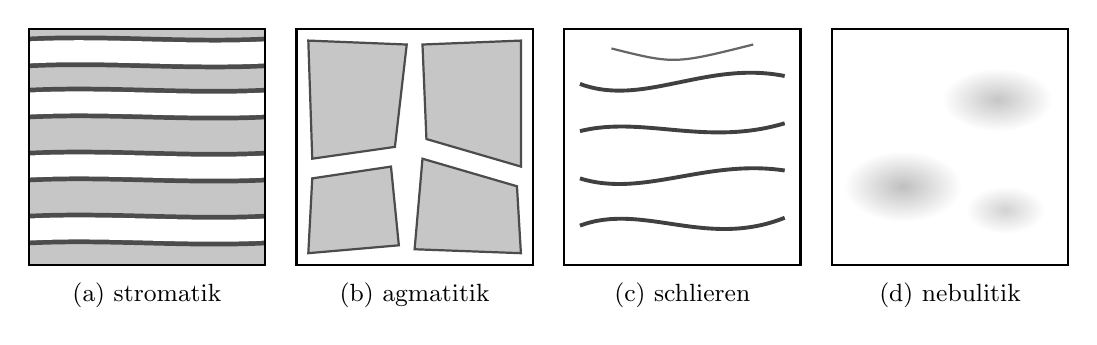
\begin{tikzpicture}[x=1cm, y=1cm]
% (a) stromatic
\begin{scope}
\fill[gray!45] (0,0) rectangle (3,3);
\foreach \y in {0.45, 1.25, 2.05, 2.7} {
  \fill[black!70] (0,\y-0.2) .. controls (1,\y-0.15) and (2,\y-0.25) .. (3,\y-0.2)
    -- (3,\y+0.2) .. controls (2,\y+0.15) and (1,\y+0.25) .. (0,\y+0.2) -- cycle;
  \fill[white] (0,\y-0.14) .. controls (1,\y-0.09) and (2,\y-0.19) .. (3,\y-0.14)
    -- (3,\y+0.14) .. controls (2,\y+0.09) and (1,\y+0.19) .. (0,\y+0.14) -- cycle;
}
\draw[thick] (0,0) rectangle (3,3);
\node[font=\small, anchor=north] at (1.5,-0.1) {(a) stromatik};
\end{scope}
% (b) agmatitic
\begin{scope}[xshift=3.4cm]
\fill[white] (0,0) rectangle (3,3);
\fill[gray!45, draw=black!70, thick] (0.15,0.15) -- (1.3,0.25) -- (1.2,1.25) -- (0.2,1.1) -- cycle;
\fill[gray!45, draw=black!70, thick] (1.5,0.2) -- (2.85,0.15) -- (2.8,1.0) -- (1.6,1.35) -- cycle;
\fill[gray!45, draw=black!70, thick] (0.2,1.35) -- (1.25,1.5) -- (1.4,2.8) -- (0.15,2.85) -- cycle;
\fill[gray!45, draw=black!70, thick] (1.65,1.6) -- (2.85,1.25) -- (2.85,2.85) -- (1.6,2.8) -- cycle;
\draw[thick] (0,0) rectangle (3,3);
\node[font=\small, anchor=north] at (1.5,-0.1) {(b) agmatitik};
\end{scope}
% (c) schlieric
\begin{scope}[xshift=6.8cm]
\fill[white] (0,0) rectangle (3,3);
\foreach \y/\a in {0.5/0.3, 1.1/-0.25, 1.7/0.2, 2.3/-0.3} {
  \draw[black!75, line width=1.4pt] (0.2,\y) .. controls (1,\y+\a) and (1.8,\y-\a) .. (2.8,\y+0.1);
}
\draw[black!60, line width=0.8pt] (0.6,2.75) .. controls (1.4,2.55) .. (2.4,2.8);
\draw[thick] (0,0) rectangle (3,3);
\node[font=\small, anchor=north] at (1.5,-0.1) {(c) schlieren};
\end{scope}
% (d) nebulitic
\begin{scope}[xshift=10.2cm]
\fill[white] (0,0) rectangle (3,3);
\shade[inner color=gray!50, outer color=white] (0.9,1.0) ellipse (0.75 and 0.45);
\shade[inner color=gray!45, outer color=white] (2.1,2.1) ellipse (0.7 and 0.4);
\shade[inner color=gray!35, outer color=white] (2.2,0.7) ellipse (0.5 and 0.3);
\draw[thick] (0,0) rectangle (3,3);
\node[font=\small, anchor=north] at (1.5,-0.1) {(d) nebulitik};
\end{scope}
\end{tikzpicture}
\par\smallskip{\small Empat struktur \omterm{def:b2:crustal-melting:migmatite}{migmatit}, skematis (bidang singkapan selebar sekitar satu
meter). Putih: \omterm{def:b2:crustal-melting:migmatite}{leukosom}; hitam: \omterm{def:b2:crustal-melting:migmatite}{melanosom}; kelabu: mesosom. (a) Stromatik: lapisan-lapisan
\omterm{def:b2:crustal-melting:migmatite}{leukosom}, masing-masing dengan tepi gelap, sejajar foliasi, khas \omterm{def:b2:crustal-melting:migmatite}{metateksit}.
(b) Agmatitik: jaringan urat \omterm{def:b2:crustal-melting:migmatite}{leukosom} di sekeliling blok-blok bersudut, yang memberi kesan
breksi. (c) Schlieren: gores-gores mineral gelap di dalam \omterm{def:b2:crustal-melting:migmatite}{leukosom}. (d) Nebulitik: bayangan samar
batuan sebelumnya di dalam massa yang tampak beku; (c) dan (d) khas
\omterm{def:b2:crustal-melting:migmatite}{diateksit}.}
\end{omfigure}
% ledger: bgs99:migmatite, scmr:migmatite

\begin{omfigure}
\centering
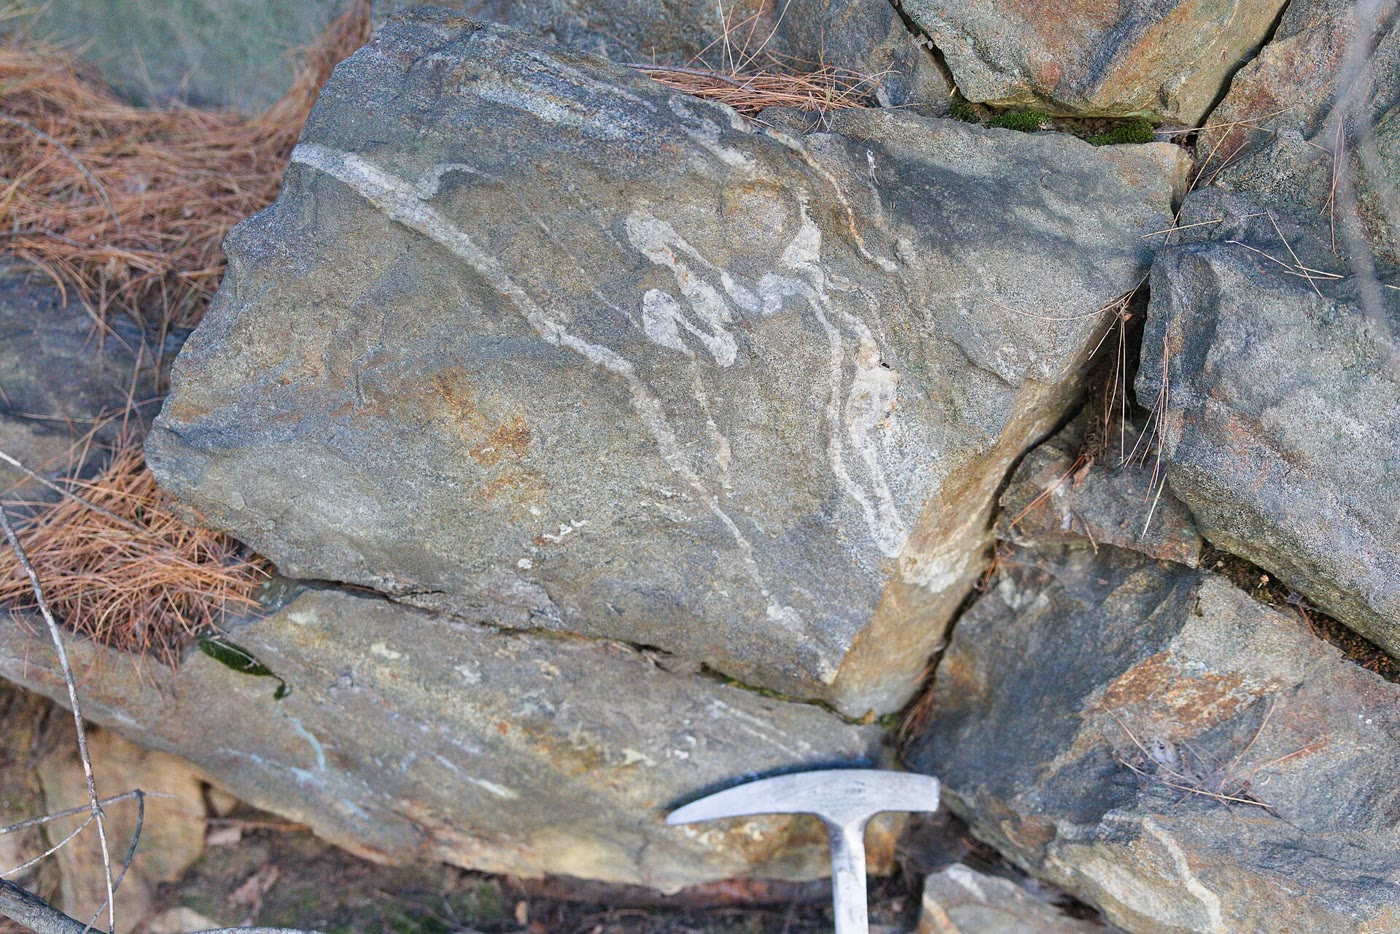
\includegraphics[width=0.62\linewidth]{images/book4/b2-12-migmatite.jpg}
\par\smallskip{\small \omterm{def:b2:crustal-melting:migmatite}{Migmatit} di Nashua, New Hampshire: urat \omterm{def:b2:crustal-melting:migmatite}{leukosom} yang terang, terlipat
bersama gneis kelabu yang mengandungnya. Palu geologi memberi skala. Foto: Kevin M. Gill, CC BY 4.0.}
\end{omfigure}

\section{Dari migmatit ke pluton}\label{sec:b2:crustal-melting:segregation}

Pada skala butir, lelehan pertama terletak di sepanjang batas butir dan dalam kantong-kantong kecil,
sebagian besar sejajar foliasi. Walaupun sedikit, lelehan itu mengubah batuan: dalam percobaan pada
granit yang meleleh sebagian, kekuatan agregatnya turun tajam antara solidus
dan \omterm{def:b2:mantle-melting:fraction}{fraksi lelehan} \num{0.07}, ketika batas-batas butir yang mengandung lelehan saling terhubung, dan turun
lagi, sekitar empat orde besaran tetapi dari nilai yang sudah rendah, ketika kerangka
kristal runtuh pada \omterm{def:b2:mantle-melting:fraction}{fraksi lelehan} yang lebih tinggi. Karena itu, kerak yang meleleh sebagian lemah,
dan deformasi terpusat di sana begitu pelelehan dimulai. Sebaliknya, deformasi menggerakkan
lelehan: lelehan mengalir keluar dari matriks di sepanjang batas butir yang terhubung ke dalam \omterm{def:b2:crustal-melting:migmatite}{leukosom} yang sejajar
foliasi, lalu keluar dari lapisan yang meleleh melalui \omterm{def:b2:crustal-melting:migmatite}{leukosom} yang memotongnya, dan
\omterm{def:b2:crustal-melting:migmatite}{leukosom-leukosom} ini bergabung menjadi \omterm{def:b2:magma-emplacement:bodies}{retas} \cref{ch:b2:magma-emplacement}. Gambar di bawah merangkum
lintasan dari sumber ke \omterm{def:b2:magma-emplacement:bodies}{pluton}.
% ledger: sawyer01:segregation, rh05:connectivity

\begin{omfigure}
\centering
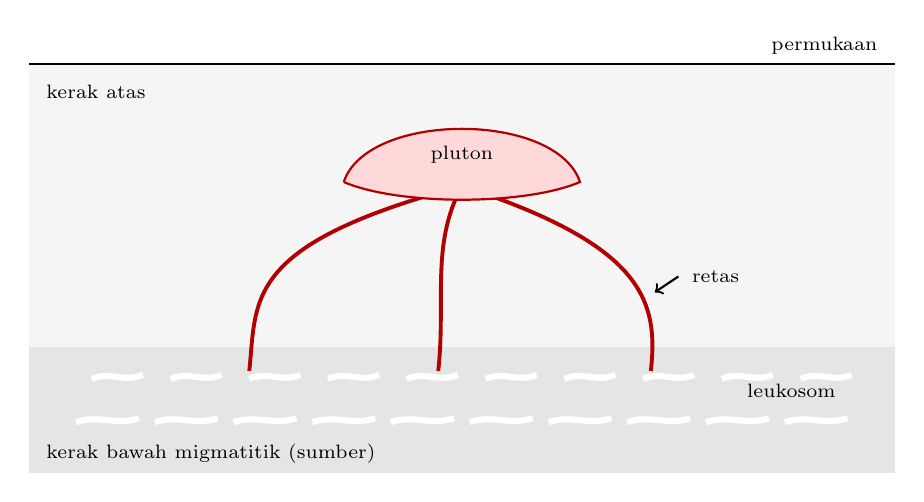
\begin{tikzpicture}[x=1cm, y=1cm]
\fill[gray!20] (0,0) rectangle (11,1.6);
\fill[gray!8] (0,1.6) rectangle (11,5.2);
\node[font=\scriptsize, anchor=west] at (0.1,0.25) {kerak bawah migmatitik (sumber)};
\foreach \x in {0.6,1.6,2.6,3.6,4.6,5.6,6.6,7.6,8.6,9.6} {
  \draw[white, line width=2.2pt] (\x,0.65) .. controls (\x+0.3,0.75) and (\x+0.5,0.6) .. (\x+0.8,0.7);
  \draw[white, line width=2.2pt] (\x+0.2,1.2) .. controls (\x+0.45,1.3) and (\x+0.6,1.15) .. (\x+0.85,1.25);
}
\foreach \x in {2.8, 5.2, 7.9} {
  \draw[red!70!black, line width=1.4pt] (\x,1.3) .. controls (\x+0.1,2.2) and (\x-0.1,2.9) .. (5.5,3.65);
}
\fill[pink!60, draw=red!70!black, thick] (4.0,3.7) .. controls (4.3,4.6) and (6.7,4.6) .. (7.0,3.7)
  .. controls (6.3,3.4) and (4.7,3.4) .. (4.0,3.7);
\node[font=\scriptsize] at (5.5,4.05) {pluton};
\node[font=\scriptsize, anchor=west] at (8.3,2.5) {retas};
\draw[->, thick] (8.25,2.5) -- (7.95,2.3);
\node[font=\scriptsize, anchor=west] at (0.1,4.85) {kerak atas};
\draw[thick] (0,5.2) -- (11,5.2);
\node[font=\scriptsize, anchor=south east] at (10.9,5.2) {permukaan};
\node[font=\scriptsize, align=left, anchor=west] at (9.0,1.05) {leukosom};
\end{tikzpicture}
\par\smallskip{\small Dari \omterm{def:b2:crustal-melting:migmatite}{migmatit} ke \omterm{def:b2:magma-emplacement:bodies}{pluton}, skematis dan tidak berskala: \omterm{def:b2:crustal-melting:migmatite}{leukosom}
(putih) di sumber yang meleleh sebagian bergabung menjadi \omterm{def:b2:magma-emplacement:bodies}{retas} (merah) yang memasok \omterm{def:b2:magma-emplacement:bodies}{pluton} yang lebih tinggi di
kerak.}
\end{omfigure}

Berapa lama kerak tetap meleleh? Di Himalaya, \omterm{def:b2:crustal-melting:anatexis}{anateksis} yang meluas dimulai sekitar
30 juta tahun setelah tumbukan India dengan Asia, dan zirkon serta monasit batuan
anatektik memberikan umur dari sekitar 25 sampai 15 juta tahun yang lalu; satu sampel dapat mencakup
sebagian besar rentang ini. Pelelehan kerak Himalaya bukanlah suatu peristiwa, melainkan suatu keadaan yang
berlangsung sekitar sepuluh juta tahun.
% ledger: weinberg16:himalaya

\section{Tipe-tipe granit}\label{sec:b2:crustal-melting:types}

Sebuah granit mengingat sumbernya dalam kimianya, terutama dalam banyaknya aluminium yang dimilikinya
dibandingkan dengan yang dapat ditampung feldsparnya.

\begin{definition}[Indeks kejenuhan aluminium]\label{def:b2:crustal-melting:asi}
Yang disebut \emph{indeks kejenuhan aluminium}\index{indeks kejenuhan aluminium} suatu batuan adalah
rasio molar
\[\mathrm{A/CNK} = \frac{n(\ce{Al2O3})}{n(\ce{CaO}) + n(\ce{Na2O}) + n(\ce{K2O})},\]
dan pendampingnya adalah $\mathrm{A/NK} = n(\ce{Al2O3})/[n(\ce{Na2O}) + n(\ce{K2O})]$. Suatu batuan
disebut \emph{peraluminus}\index{peraluminus} jika $\mathrm{A/CNK} > 1$,
\emph{metaluminus}\index{metaluminus} jika $\mathrm{A/CNK} < 1 < \mathrm{A/NK}$, dan
\emph{peralkalin}\index{peralkalin} jika $\mathrm{A/NK} < 1$.
\end{definition}
% ledger: moyen17:aluminosity, frost01:asi

\begin{proposition}[Apa yang diukur indeks itu]\label{prop:b2:crustal-melting:feldspar}
Batuan yang seluruh kalsium, natrium, dan kaliumnya berada dalam feldspar, dan yang seluruh aluminiumnya
berada dalam feldspar, memiliki $\mathrm{A/CNK} = 1$. Karena itu, batuan \omterm{def:b2:crustal-melting:asi}{peraluminus} memiliki sisa aluminium
setelah feldsparnya, yang ditampung dalam mineral beraluminium (muskovit, garnet, kordierit,
aluminosilikat); batuan \omterm{def:b2:crustal-melting:asi}{metaluminus} memiliki sisa kalsium, yang ditampung dalam silikat kalsium
(hornblende, klinopiroksen, titanit); dan batuan \omterm{def:b2:crustal-melting:asi}{peralkalin} memiliki sisa natrium dan kalium,
yang ditampung dalam mineral yang aluminiumnya tidak cukup untuk feldspar (piroksen natrium dan
amfibol natrium).
\end{proposition}

\begin{proof}
Dalam bentuk oksida, K-feldspar adalah \ce{K2O.Al2O3.6SiO2}, albit \ce{Na2O.Al2O3.6SiO2}, dan
anortit \ce{CaO.Al2O3.2SiO2}: setiap rumus memiliki tepat satu \ce{Al2O3} untuk satu
\ce{K2O}, \ce{Na2O}, atau \ce{CaO}. Karena itu, setiap campuran ketiganya memiliki $n(\ce{Al2O3}) =
n(\ce{CaO}) + n(\ce{Na2O}) + n(\ce{K2O})$, yaitu $\mathrm{A/CNK} = 1$. Jika
$\mathrm{A/CNK} > 1$, aluminiumnya melebihi yang dapat diikat alkali dan kalsium menjadi
feldspar, dan kelebihannya pasti berada dalam mineral lain. Jika $\mathrm{A/CNK} < 1$ tetapi
$\mathrm{A/NK} > 1$, aluminium cukup untuk seluruh natrium dan kalium sebagai
feldspar tetapi tidak untuk seluruh kalsium, yang masuk ke mineral yang memerlukan lebih sedikit aluminium
per kalsium daripada anortit. Jika $\mathrm{A/NK} < 1$, bahkan alkali pun tidak dapat seluruhnya berada dalam
feldspar.
\end{proof}

Moyen dan kawan-kawan mendapati aluminositas sebagai indikator yang paling berguna untuk membedakan granit
dengan sumber yang berbeda; Frost dan kawan-kawan memakai indeks yang sama, dengan sedikit
koreksi untuk fosfor, sebagai salah satu dari tiga sumbu klasifikasi batuan granitik
mereka.
% ledger: moyen17:aluminosity, frost01:asi

\begin{omfigure}
\centering
\begin{tikzpicture}
\begin{axis}[omrecord, width=0.72\linewidth, height=7cm,
  xmin=0.4, xmax=1.5, ymin=0.4, ymax=3.5, xlabel={A/CNK (rasio molar)}, ylabel={A/NK (rasio molar)},
  tick label style={font=\scriptsize}, label style={font=\small}]
\addplot[fill=gray!15, draw=none] coordinates {(0.4,0.4) (1.5,1.5) (1.5,0.4) (0.4,0.4)};
\addplot[thick, black!70] coordinates {(1,0.4) (1,3.5)};
\addplot[thick, black!70] coordinates {(0.4,1) (1.5,1)};
\node[font=\scriptsize, anchor=north east] at (axis cs:1.48,3.45) {peraluminus};
\node[font=\scriptsize, anchor=west] at (axis cs:0.62,2.6) {metaluminus};
\node[font=\scriptsize, anchor=south west] at (axis cs:0.42,0.45) {peralkalin};
\addplot[only marks, mark=*, mark size=2pt, blue!70!black, nodes near coords,
  point meta=explicit symbolic, every node near coord/.style={font=\scriptsize, anchor=west}]
  coordinates {(0.539,3.196)[BHVO-2] (0.877,1.694)[AGV-2] (0.993,1.135)[SRM 278]};
\addplot[only marks, mark=square*, mark size=2pt, red!70!black]
  coordinates {(1.261,1.377) (0.809,0.844)};
\node[font=\scriptsize, red!70!black, anchor=south] at (axis cs:1.261,1.45) {lelehan tipe-S};
\node[font=\scriptsize, red!70!black, anchor=north] at (axis cs:0.809,0.79) {granit peralkalin};
\end{axis}
\end{tikzpicture}
\par\smallskip{\small Diagram Shand. Lingkaran biru: tiga bahan acuan, basal
Hawaii (BHVO-2), andesit (AGV-2), dan obsidian berkomposisi granitik (SRM 278),
yang dihitung dari kadar oksida terbitannya. Kotak merah: dua granit rekaan yang dipakai dalam
bab ini. Segitiga kelabu tidak dapat dicapai, karena A/CNK tidak pernah melebihi A/NK.}
\end{omfigure}
% ledger: usgs:bhvo2-major, usgs:agv2-major, nist278:majors

Kimia mengikuti sumbernya. Pada 1974, Chappell dan White memperhatikan bahwa, selain batuan yang
paling felsik, granit-granit Sabuk Lipatan Lachlan terbagi menjadi dua kelompok yang berbeda jelas,
dan menafsirkannya sebagai lelehan dua jenis batuan sumber: batuan beku yang lebih tua dan batuan sedimen. Hidrolisis feldspar, yang dibahas dalam volume Tahun 1,
mengangkut natrium dan kalsium dalam larutan dan menahan aluminium dalam lempung: lumpur yang terbuat
dari lempung ini kaya aluminium, demikian pula lelehannya.
% ledger: cw01:is-types

\begin{definition}[Tipologi granit]\label{def:b2:crustal-melting:types}
Yang disebut \emph{granit tipe-I}\index{granit tipe-I} adalah granit yang sumbernya terutama
batuan beku yang lebih tua, \emph{granit tipe-S}\index{granit tipe-S} adalah granit yang sumbernya
terutama batuan sedimen (metasedimen), dan granit tipe-M adalah granit yang berasal dari
mantel. Yang disebut \emph{granit tipe-A}\index{granit tipe-A} didefinisikan oleh kimia dan
tatanannya, bukan oleh sumbernya: kaya besi dan kalium, sangat diperkaya \omterm{def:b2:elements-in-the-earth:partition}{unsur
inkompatibel}, dan ditempatkan dalam tatanan intralempeng yang stabil, busur belakang, atau pascatumbukan.
\end{definition}
% ledger: johansson23:a-type, cw01:is-types

\omterm{def:b2:crustal-melting:types}{Granit tipe-S} bersifat \omterm{def:b2:crustal-melting:asi}{peraluminus}, dengan dua mika atau dengan kordierit; granitoid tipe-A
sebagian besar \omterm{def:b2:crustal-melting:asi}{metaluminus}, sebagian \omterm{def:b2:crustal-melting:asi}{peraluminus}. Akan tetapi, satu analisis saja dapat menyesatkan: setiap
rangkaian granitoid berakhir di dekat komposisi minimum granitik, leukokratik dan sedikit
\omterm{def:b2:crustal-melting:asi}{peraluminus}, sehingga sampel \omterm{def:b2:crustal-melting:asi}{peraluminus} bukanlah bukti bahwa keraklah yang meleleh. Yang membedakan
rangkaian-rangkaian itu adalah bentuk trennya dalam diagram Shand: rangkaian busur mencapai
minimum itu di sepanjang larik curam dari A/NK tinggi dan A/CNK rendah, rangkaian tipe-S berkalsium rendah
di sepanjang larik dengan A/NK mendekati A/CNK. Belum ada kesepakatan tentang sumber
\omterm{def:b2:magma-emplacement:magma}{magma} tipe-A: salah satu model membentuknya dari basal hasil underplating, yang berevolusi melalui kristalisasi,
\omterm{def:b2:mantle-melting:melting}{pelelehan sebagian}, dan \omterm{def:b2:magmatic-differentiation:open}{asimilasi kerak}.
% ledger: moyen17:trends, frost01:asi, johansson23:a-type

\begin{definition}[Leukogranit]\label{def:b2:crustal-melting:leucogranite}
Yang disebut \emph{leukogranit}\index{leukogranit} adalah granit berwarna terang, yang hampir bebas
mineral gelap; leukogranit \omterm{def:b2:crustal-melting:asi}{peraluminus} sabuk tumbukan mengandung muskovit, sendiri atau
bersama biotit.
\end{definition}
% ledger: moyen17:aluminosity, pdh98:himalaya

\omterm{def:b2:crustal-melting:leucogranite}{Leukogranit} \omterm{def:b2:crustal-melting:asi}{peraluminus} bermuskovit di sabuk tumbukan memiliki komposisi yang dekat
dengan cairan pelelehan dengan air atau \omterm{def:b2:crustal-melting:reactions}{pelelehan dehidrasi} muskovit, pada suhu di dekat
\qty{700}{\celsius} tempat zirkon dan monasit sumbernya dapat bertahan dan terbawa
ke dalam lelehan sebagai xenokris; granit \omterm{def:b2:crustal-melting:asi}{peraluminus} berkordierit berasal dari
penguraian biotit yang lebih panas, pada 800 sampai \qty{850}{\celsius}. \omterm{def:b2:crustal-melting:leucogranite}{Leukogranit} Himalaya,
dengan tanda isotop kerak yang kuat, termasuk keluarga ini
(\cref{ch:b2:himalaya-andes}).
% ledger: moyen17:aluminosity, weinberg16:himalaya

\begin{omfigure}
\centering
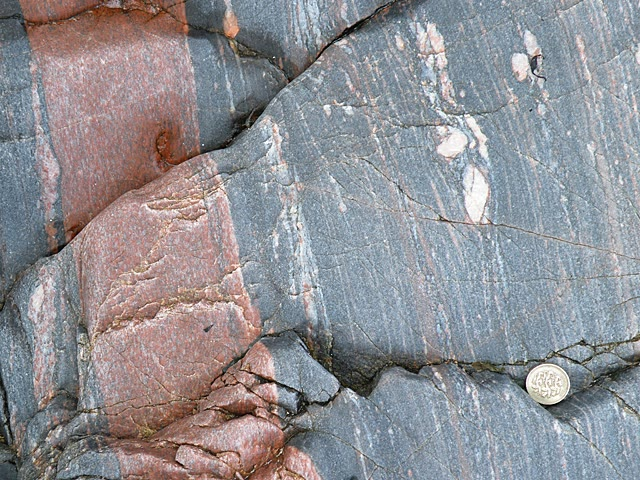
\includegraphics[width=0.5\linewidth]{images/book4/b2-12-leucogranite-vein.jpg}
\par\smallskip{\small Urat \omterm{def:b2:crustal-melting:leucogranite}{leukogranit} merah muda yang memotong gneis kelabu berlapis; koin memberi
skala. Foto: Anne Burgess (Geograph), CC BY-SA 2.0.}
\end{omfigure}

\section{Granit dan pertumbuhan benua}\label{sec:b2:crustal-melting:time}

Ada dua jenis tempat yang menghasilkan sebagian besar granit. Di atas zona subduksi, kerak busur terbentuk melalui
diferensiasi lelehan mafik dari mantel, dan panas yang tersedia hanyalah yang dibawa
lelehan itu. Setelah tumbukan, kerak yang menebal adalah sistem yang sangat panas: kerak itu meleleh dalam
skala besar, pada suhu rendah bila air atau muskovit memungkinkannya dan pada suhu lebih
tinggi melalui penguraian biotit, dan granit-granit yang berasal dari kerak ini mendaur ulang kerak yang
sudah ada. Lelehan mantel juga mencapai kerak di sana, dalam jumlah yang cukup besar, menurut Moyen dan
kawan-kawan, untuk menjadikan sabuk orogen tahap akhir penyumbang penting bagi pertumbuhan
kerak. Apakah sebuah granit menambah benua atau hanya mengolahnya kembali dengan demikian adalah persoalan
sumbernya, yang dijawab oleh isotopnya (\cref{ch:b2:isotope-geochemistry}); granit-granit
Bumi purba, yang sangat berbeda dari granit-granit ini, adalah pokok bahasan
\cref{ch:b2:precambrian-earth}.
% ledger: moyen17:settings

\section{Latihan}\label{sec:b2:crustal-melting:exercises}

Massa molar (\unit{\gram\per\mole}): \ce{Al2O3} 101.96, \ce{CaO} 56.08, \ce{Na2O} 61.98,
\ce{K2O} 94.20, \ce{H2O} 18.02; massa atom: H 1.008, O 16.00, Na 22.99, Mg 24.31,
Al 26.98, Si 28.09, K 39.10, Ca 40.08. Ambillah $g = \qty{9.81}{\metre\per\second\squared}$.

\begin{exercise}[$\star$]\label{exo:b2:crustal-melting:1}
Bahan acuan andesit AGV-2 mengandung, dalam \unit{\gram} per \qty{100}{\gram},
\ce{Al2O3} 17.03, \ce{CaO} 5.15, \ce{Na2O} 4.204, dan \ce{K2O} 2.898.
(a) Hitunglah A/CNK dan A/NK-nya. (b) Klasifikasikan batuan itu, dan sebutkan satu mineral yang seharusnya menampung
kelebihan kalsiumnya.
\end{exercise}
% ledger: usgs:agv2-major

\begin{exercise}[$\star$]\label{exo:b2:crustal-melting:2}
Tiga granit mengandung, selain kuarsa dan feldspar: (a) muskovit, biotit, dan garnet;
(b) hornblende, biotit, dan titanit; (c) egirin, piroksen natrium--besi
\ce{NaFeSi2O6}, dan amfibol natrium. Klasifikasikan masing-masing menurut kejenuhan aluminiumnya, dan sebutkan
mana yang dapat berupa \omterm{def:b2:crustal-melting:types}{granit tipe-S}.
\end{exercise}

\begin{exercise}[$\star$]\label{exo:b2:crustal-melting:3}
Kerak bermassa jenis \qty{2800}{\kilogram\per\cubic\metre} memiliki geoterm linear
$T = \qty{10}{\celsius} + (\qty{20}{\celsius\per\kilo\metre})\,z$. Antara 2 dan
\qty{10}{kbar}, dekatilah solidus granit basah dengan garis lurus yang melalui
(\qty{680}{\celsius}, \qty{2}{kbar}) dan (\qty{620}{\celsius}, \qty{10}{kbar}). Pada kedalaman,
suhu, dan tekanan berapa geoterm itu memotongnya?
\end{exercise}
% ledger: sw81:wet-solidus

\begin{exercise}[$\star$]\label{exo:b2:crustal-melting:4}
Sebuah gneis biotit kelabu mengandung lapisan putih kuarsa dan feldspar setebal sentimeter, yang sejajar
foliasinya, masing-masing dibatasi oleh jalur hitam tipis biotit; di antara lapisan-lapisan itu
gneisnya tampak biasa. (a) Namailah lapisan putih, jalur hitam, dan gneis yang biasa.
(b) Apakah batuan itu \omterm{def:b2:crustal-melting:migmatite}{metateksit} atau \omterm{def:b2:crustal-melting:migmatite}{diateksit}, dan apa strukturnya? (c) Beberapa ratus
meter dari situ, perlapisannya telah hilang: batuan bergores yang mirip granit mengandung bayangan samar
gneis. Apa yang telah berubah?
\end{exercise}
% ledger: scmr:migmatite, bgs99:migmatite

\begin{exercise}[$\star\star$]\label{exo:b2:crustal-melting:5}
Anggaplah biotit sebagai flogopit, \ce{KMg3AlSi3O10(OH)2}. (a) Hitunglah massa molarnya dan
fraksi massa air yang dilepaskannya (kedua gugus hidroksilnya menghasilkan satu \ce{H2O}).
(b) Sebuah gneis dengan \qty{25}{\percent} massa biotit meleleh melalui \omterm{def:b2:crustal-melting:reactions}{pelelehan dehidrasi} biotit
menjadi lelehan yang mengandung \qty{4.0}{\percent} air. Dengan
\cref{prop:b2:crustal-melting:water}, tentukan \omterm{def:b2:mantle-melting:fraction}{fraksi lelehannya}, dan bandingkan dengan
fraksi yang didapat dalam percobaan \omterm{def:b2:crustal-melting:reactions}{pelelehan dehidrasi} biotit.
\end{exercise}
% ledger: bk99:migmatites

\begin{exercise}[$\star\star$]\label{exo:b2:crustal-melting:6}
Seratus gram granit mengandung \qty{30}{\gram} K-feldspar \ce{KAlSi3O8},
\qty{35}{\gram} albit \ce{NaAlSi3O8}, \qty{5}{\gram} anortit \ce{CaAl2Si2O8},
\qty{25}{\gram} kuarsa, dan \qty{5}{\gram} muskovit \ce{KAl3Si3O10(OH)2}.
(a) Hitunglah massa molar keempat mineral beraluminium itu. (b) Hitunglah jumlah
\ce{Al2O3}, \ce{CaO}, \ce{Na2O}, dan \ce{K2O} dalam batuan itu, serta A/CNK-nya. (c) Mineral
mana yang membuat batuan itu \omterm{def:b2:crustal-melting:asi}{peraluminus}?
\end{exercise}

\begin{exercise}[$\star\star$]\label{exo:b2:crustal-melting:7}
Sebuah \omterm{def:b2:magma-emplacement:bodies}{sill} basaltik yang terintrusi pada \qty{1200}{\celsius} mengkristal sepenuhnya dan mendingin sampai
\qty{850}{\celsius}, sambil melepaskan panas laten \qty{900}{\mega\joule\per\cubic\metre}.
Kerak di sekelilingnya, pada \qty{650}{\celsius}, terpanaskan sampai \qty{850}{\celsius} dan
\qty{20}{\percent} di antaranya meleleh, dengan panas laten per satuan volume lelehan yang sama. Kedua
batuan memiliki kapasitas kalor \qty{2.5}{\mega\joule\per\cubic\metre\per\kelvin}. Dengan
\cref{prop:b2:crustal-melting:heat}, berapa meter kubik kerak yang dapat diolah dengan cara ini oleh satu meter kubik
basal? Apa yang diabaikan hasil itu?
\end{exercise}
% ledger: delaney86b4:properties

\begin{exercise}[$\star\star$]\label{exo:b2:crustal-melting:8}
Bahan acuan obsidian SRM 278 disertifikasi dengan \ce{Al2O3}
$14.15 \pm 0.15$, \ce{CaO} 0.983, \ce{Na2O} 4.84, dan \ce{K2O} 4.16 (\unit{\percent}
massa). (a) Hitunglah A/CNK dan A/NK-nya, lalu klasifikasikan. (b) Hitung ulang A/CNK dengan kedua
ujung ketidakpastian \ce{Al2O3}. Apakah klasifikasinya kokoh?
\end{exercise}
% ledger: nist278:majors

\begin{exercise}[$\star\star$]\label{exo:b2:crustal-melting:9}
Pada \qty{800}{\celsius}, lelehan haplogranit yang jenuh air mengandung \qty{7.45}{\percent}
air pada \qty{3}{kbar}, 8.94 pada \qty{4}{kbar}, 9.97 pada \qty{5}{kbar}, dan 13.82 pada
\qty{8}{kbar}. (a) Cocokkan garis lurus pada keempat titik ini dengan kuadrat terkecil dan bandingkan
kemiringannya dengan \qty{1.27}{\percent} per kilobar yang dikutip para peneliti percobaan itu.
(b) Ramalkan kadar jenuh pada \qty{6}{kbar}. (c) Berapa massa lelehan terkecil
yang dapat membawa \qty{10}{\gram} air pada \qty{6}{kbar}? (d) Mengapa garis itu tidak boleh
dipakai pada \qty{15}{kbar}?
\end{exercise}
% ledger: holtz95:solubility

\begin{exercise}[$\star\star\star$]\label{exo:b2:crustal-melting:10}
Dekatilah solidus \omterm{def:b2:crustal-melting:reactions}{pelelehan dehidrasi} sekis muskovit dengan garis lurus yang melalui
(\qty{750}{\celsius}, \qty{6}{kbar}) dan (\qty{800}{\celsius}, \qty{10}{kbar}),
ujung-ujung rentang eksperimental. Sebuah sekis pada \qty{770}{\celsius} naik dari
\qty{10}{kbar} tanpa menerima atau kehilangan panas. (a) Pada tekanan berapa sekis itu mencapai
solidus? (b) Selanjutnya, suhunya mengikuti solidus turun, dan panas untuk pelelehan berasal
dari pendinginannya sendiri. Dengan kapasitas kalor \qty{2.5}{\mega\joule\per\cubic\metre\per\kelvin}
dan panas laten \qty{900}{\mega\joule\per\cubic\metre}, berapa fraksi volume lelehan
yang telah terbentuk ketika sekis itu mencapai \qty{6}{kbar}? (c) Bandingkan dengan kondisi yang diajukan untuk
\omterm{def:b2:crustal-melting:leucogranite}{leukogranit} Himalaya.
\end{exercise}
% ledger: pdh98:himalaya, delaney86b4:properties

\begin{exercise}[$\star\star\star$]\label{exo:b2:crustal-melting:11}
Panas berdifusi sejauh $\ell$ dalam waktu berorde $\ell^2/\kappa$. Dengan
$\kappa = \qty{1e-6}{\square\metre\per\second}$, taksirlah waktu yang diperlukan panas sebuah \omterm{def:b2:magma-emplacement:bodies}{sill}
setebal \qty{2}{km}, dan sebuah lapisan underplating setebal \qty{10}{km}, untuk menyebar sejauh
tebalnya sendiri. Bandingkan dengan sepuluh juta tahun \omterm{def:b2:crustal-melting:anatexis}{anateksis} Himalaya: dapatkah satu
peristiwa underplating menjelaskannya?
\end{exercise}
% ledger: delaney86b4:properties, weinberg16:himalaya

\begin{exercise}[$\star\star\star$]\label{exo:b2:crustal-melting:12}
Sebuah \omterm{def:b2:crustal-melting:migmatite}{migmatit} stromatik dianalisis: \omterm{def:b2:crustal-melting:migmatite}{leukosom} \ce{K2O} \qty{5.0}{\percent}, \ce{MgO}
\qty{0.20}{\percent}; \omterm{def:b2:crustal-melting:migmatite}{melanosom} \ce{K2O} \qty{2.0}{\percent}, \ce{MgO}
\qty{4.0}{\percent}; mesosom, yang dianggap sebagai batuan induk yang tidak meleleh, \ce{K2O}
\qty{2.75}{\percent}, \ce{MgO} \qty{3.05}{\percent} (semuanya persen massa). (a) Jika
neosom terbentuk dari batuan induk tanpa penambahan atau kehilangan, berapa fraksi massanya yang berupa
\omterm{def:b2:crustal-melting:migmatite}{leukosom}? (b) Periksalah jawaban itu dengan \ce{MgO}. (c) Di singkapan, \omterm{def:b2:crustal-melting:migmatite}{leukosom} hanya membentuk
\qty{10}{\percent} massa neosom. Berapa gram lelehan yang pergi per
\qty{100}{\gram} batuan induk?
\end{exercise}

\begin{problem}[{Soal akhir pekan --- sebuah pluton dari mika yang meleleh}]\label{pb:b2:crustal-melting:1}
Sebuah sekis yang terdiri atas \qty{20}{\percent} muskovit, \qty{15}{\percent} biotit,
\qty{30}{\percent} kuarsa, \qty{30}{\percent} plagioklas, dan \qty{5}{\percent} mineral
lain (persen massa; batuan rekaan) terletak di dasar kerak yang digandakan oleh penumpukan, yaitu
situasi yang dimodelkan dalam \cref{ch:b2:pt-paths}. Sekis itu dapat meleleh dan memasok sebuah \omterm{def:b2:magma-emplacement:bodies}{pluton} granit. Data:
massa atom dan massa molar di awal latihan; solidus granit basah melalui
(\qty{680}{\celsius}, \qty{2}{kbar}), (\qty{620}{\celsius}, \qty{10}{kbar}),
(\qty{605}{\celsius}, \qty{15.3}{kbar}), dan (\qty{670}{\celsius}, \qty{27}{kbar}); kadar
jenuh air lelehan granitik pada \qty{800}{\celsius} adalah \qty{9.97}{\percent} pada
\qty{5}{kbar} dan \qty{13.82}{\percent} pada \qty{8}{kbar}. Dasar kerak yang menebal dalam model itu mengikuti:

\smallskip
\begin{center}\small
\begin{tabular}{l|ccccccccccc}
$t$ (\unit{Ma}) & 0 & 10 & 20 & 30 & 40 & 50 & 60 & 70 & 80 & 90 & 100\\ \hline
$T$ (\unit{\celsius}) & 595 & 656 & 734 & 795 & 845 & 885 & 909 & 914 & 900 & 867 & 814\\
$P$ (\unit{kbar}) & 19.2 & 19.2 & 19.2 & 19.2 & 17.9 & 16.5 & 15.1 & 13.7 & 12.4 & 11.0 & 9.6
\end{tabular}
\end{center}
\smallskip

\noindent\textbf{Bagian I --- Air dari mika.}
\begin{enumerate}
\item Hitunglah massa molar muskovit \ce{KAl3Si3O10(OH)2}.
\item Kedua gugus hidroksilnya menghasilkan satu \ce{H2O}. Berapa fraksi massa mineral itu yang
dilepaskan sebagai air?
\item Berapa banyak air yang dilepaskan muskovit dalam satu kilogram sekis?
\item Dengan interpolasi linear, berapa kadar air jenuh lelehan pada
\qty{7}{kbar}? Berapa \omterm{def:b2:mantle-melting:fraction}{fraksi lelehan} terkecil yang dapat dihasilkan air muskovit itu?
\item Lelehan hasil \omterm{def:b2:crustal-melting:reactions}{pelelehan dehidrasi} jauh dari jenuh; ambillah kadar airnya
\qty{6.0}{\percent}. Berapa \omterm{def:b2:mantle-melting:fraction}{fraksi lelehan} yang dihasilkan muskovit?
\item Dalam percobaan pada \omterm{def:b2:metamorphic-facies:protoliths}{metapelit} dua mika pada \qty{10}{kbar}, reaksi muskovit
hanya menghasilkan 1 sampai \qty{2}{\percent} lelehan. Sebutkan dua alasan mengapa batuan yang sebenarnya dapat menghasilkan lebih sedikit
lelehan daripada jawabanmu untuk pertanyaan~5.
\end{enumerate}

\noindent\textbf{Bagian II --- Memanaskan sumbernya.}
\begin{enumerate}[resume]
\item Dalam \cref{ch:b2:pt-paths}, batuan yang tertinggal di kerak tengah mencapai puncak pada \qty{593}{\celsius}
dan \qty{7.8}{kbar}. Berapa solidus basah pada \qty{7.8}{kbar}? Dapatkah batuan itu meleleh, bahkan
dengan air bebas?
\item Dengan interpolasi antara 15.3 dan \qty{27}{kbar}, tentukan solidus basah pada tekanan
dasar kerak tepat setelah penumpukan. Apakah dasar itu berada di atasnya pada $t = 0$? Pada $t = \qty{10}{Ma}$?
\item Apa yang membatasi pelelehan dasar kerak pada $t = \qty{10}{Ma}$, dan mengapa pelelehan itu segera
berhenti?
\item Kapan dasar kerak melewati \qty{800}{\celsius}, ujung atas rentang
muskovit?
\item Rentang amfibol mencakup 875 sampai \qty{925}{\celsius} pada 10 sampai \qty{12.5}{kbar}.
Kapan dasar kerak memasuki rentang tekanan ini, dan pada suhu berapa?
\item Kapan dasar kerak mencapai \qty{10}{kbar}, batas atas rentang tekanan
percobaan muskovit, dan seberapa panas dasar itu saat itu? Mineral hidrus mana dalam sekis itu yang
masih dapat ada?
\end{enumerate}

\noindent\textbf{Bagian III --- Lelehan apa?}
Setelah mengkristal, lelehan itu menghasilkan \omterm{def:b2:crustal-melting:leucogranite}{leukogranit} (analisis rekaan) dengan, dalam
\unit{\percent} massa, \ce{Al2O3} 15.0, \ce{CaO} 0.55, \ce{Na2O} 3.4, dan \ce{K2O} 4.9.
\begin{enumerate}[resume]
\item Hitunglah jumlah keempat oksida itu dalam \qty{100}{\gram} batuan.
\item Hitunglah A/CNK-nya.
\item Hitunglah A/NK-nya dan klasifikasikan \omterm{def:b2:crustal-melting:leucogranite}{leukogranit} itu.
\item Apakah granit itu bertipe-I atau bertipe-S? Sebutkan dua mineral yang seharusnya menampung kelebihan
aluminiumnya.
\item Berapa mol \ce{Al2O3} per \qty{100}{\gram} yang tersisa setelah
feldspar? Jika semuanya masuk ke muskovit, yang mengandung satu \ce{Al2O3} lebih banyak per satuan
rumus daripada K-feldspar, berapa gram muskovit yang akan terkandung dalam \qty{100}{\gram} granit?
\item Obsidian SRM 278 memiliki A/CNK $= 0.993$. Dapatkah \omterm{def:b2:crustal-melting:leucogranite}{leukogranit} dan obsidian itu
berasal dari jenis sumber yang sama?
\end{enumerate}

\noindent\textbf{Bagian IV --- Berapa banyak kerak?}
Sebuah \omterm{def:b2:magma-emplacement:bodies}{pluton} rekaan dari \omterm{def:b2:crustal-melting:leucogranite}{leukogranit} ini bervolume \qty{1000}{\cubic\kilo\metre}.
Ambillah \qty{2650}{\kilogram\per\cubic\metre} untuk granit dan
\qty{2800}{\kilogram\per\cubic\metre} untuk sekis; andaikan \qty{70}{\percent}
lelehan meninggalkan sumbernya dan seluruh air lelehan keluar ketika lelehan itu mengkristal.
\begin{enumerate}[resume]
\item Berapa massa \omterm{def:b2:magma-emplacement:bodies}{pluton} itu?
\item Berapa massa lelehan (dengan \qty{6.0}{\percent} airnya) yang diperlukannya?
\item Dengan \omterm{def:b2:mantle-melting:fraction}{fraksi lelehan} pertanyaan~5, berapa massa sekis yang harus meleleh?
\item Berapa volume sekis itu?
\item Jika sumbernya berupa lapisan setebal \qty{5}{km}, seberapa luas daerah yang meleleh?
\item Jika yang dipakai adalah \omterm{def:b2:mantle-melting:fraction}{fraksi lelehan} terkecil pertanyaan~4, berapa kali lebih besar sumbernya?
Berikan volume kerak sumber yang meleleh untuk membentuk \omterm{def:b2:magma-emplacement:bodies}{pluton} itu, dalam
\unit{\cubic\kilo\metre}, dari pertanyaan~22.
\end{enumerate}
\end{problem}
